% Framework:
% \begin{itemize}
%     \item Tool learning empowers LLM.
%     \item However, how to benchmark LLMs on tool usage remains an open issue. There exists a trade-off between questioning reality (To Be Defined/Changed) and the number of APIs but real-life tool using needs both. Previous works fall on one side.
%     \item We propose a new benchmark that strikes a balance between them. including scenario-based question construction, cache-based large-scale API pool and query satisfaction-oriented evaluation. We also propose a new strong baseline....
% \end{itemize}
% \textbf{\textcolor{red}{Framework:}}


% Large Language Models (LLMs, \citealp{brown2020language, geminiteam2023gemini,openai2023gpt4, touvron2023llama}) have demonstrated considerable achievements across a diverse array of tasks, such as commonsense reasoning~\cite{weng2023large, ling2023deductive} and coding~\cite{chen2021evaluating, rozière2023code}. When augmented with auxiliary tools including online search engines and external computational models, LLMs demonstrate enhanced performance in more complex tasks~\cite{nakano2022webgpt, yao2023react, lu2023chameleon}. Therefore, at the time when tool learning becomes more powerful, benchmarking LLMs in the context of tool learning has been increasingly important.

With the rapid developments of Large Language Models (LLMs; \citealp{brown2020language, geminiteam2023gemini,openai2023gpt4, touvron2023llama}), tool learning which leverage LLMs to schedule a variety of external tools has attracted enormous attention~\cite{nakano2022webgpt, yao2023react, lu2023chameleon}.
\blfootnote{Project: 
\href{https://zhichengg.github.io/stb.github.io/}{\texttt{zhichengg.github.io/stb.github.io/}}}\blfootnote{GitHub: \href{https://github.com/THUNLP-MT/StableToolBench}{\texttt{THUNLP-MT/StableToolBench}}} 
Previous studies~\citep{hao2023toolkengpt, hsieh2023tool, schick2023toolformer, tang2023toolalpaca} aim to augment LLMs with tools to enhance performance on conventional natural language processing (NLP) downstream tasks, while recent work~\citep{qin2023webcpm, NEURIPS2022_82ad13ec_webshop, cai2024large} primarily focus on solving real-world scenarios that require the use of tools.
In general, tool learning complements the capabilities of vanilla LLMs and bridges the gap to real-world applications.


To assess the capability of LLMs to use tools, a series of tool learning benchmarks have been introduced. 
Several pioneering studies have heavily relied on human-crafted offline tools~\cite{gpt4tools, xu2023tool} or hand-selected online tools~\cite{li2023api, li2023apibank, chen2023teval}.
While these tools are high-quality, their scale remains relatively small, thereby limiting their ability to accurately reflect real-world scenarios.
To address this limitation, subsequent studies~\citep{tang2023toolalpaca, ye2024tooleyes, qin2023tool} have advocated for leveraging extensive collections of online tools that span across various domains.
Owing to the increased scale, the automatic evaluation of tool learning has moved closer to real-world scenarios.
However, concerns have been raised regarding the stability of these online tools, which has implications for the reproducibility and comparability of benchmark performance over time\footnote{According to its \href{https://www.oed.com/dictionary/benchmark_n?tab=meaning_and_use}{definition}, benchmarks should remain stable, and the model performance assessed on them must be comparable over time.}. 
For instance, the well-recognised ToolBench\footnote{We use  ToolEval2 in ToolBench as the benchmark.}~\cite{qin2023toolllm} has shown performance discrepancies that cannot be reproduced months after its release, as analysed in ~\Cref{sec:pre_analysis_performance}.
This is even more important when faced with a complex environment, where APIs and tools keep changing while the evaluation should maintain its consistency across time.
% For example, ToolBench~\cite{qin2023toolllm}~\footnotemark[1] and ToolEyes~\cite{ye2024tooleyes} exploit real online tools to make up queries covering various domains for evaluation.
% There exists an impossible triangle between benchmark stability, tool reality and the scalability of the the benchmark. Benchmarks equipped with a large number of real tools or APIs tend to be less stable because these tools can change over time. As a result, performance of a model at different time can be different.
% On the other hand, stable offline tools, relied on manual creation, are often limited in narrow scenarios, which makes it even harder to curate real-world questions.
% One can also manually filter out stable real online APIs. However, this tasks a lot of labor work, resulting in small dataset size  and number of tools.
% \footnotetext[1]{For differentiation, we denote ToolBench for ToolBench~\cite{qin2023toolllm} and ToolBench-X for ToolBench~\cite{xu2023tool} below.}

% \begin{figure}
%     \centering
%     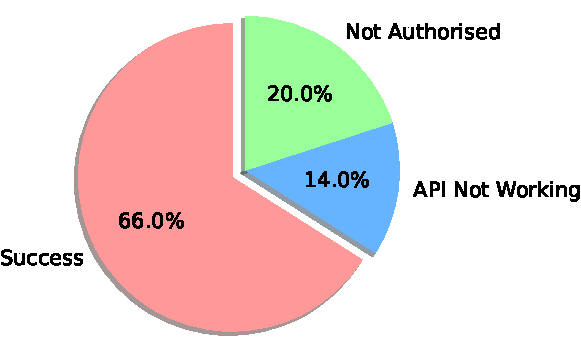
\includegraphics[width=\linewidth]{figs/toolbench_api_statistics.pdf}
%     \caption{API calling statistics in ToolBench. We randomly sample 50 APIs to test the health of these APIs. \textcolor{red}{Add ToolEyes.}}
%     \label{fig:api_statistics}
% \end{figure}

% \begin{minipage}{\textwidth}
% \begin{table*}
%     \centering
%     \resizebox{\linewidth}{!}{
%     \begin{tabular}{lrrcccc}
%         \toprule
%         {\textbf{Benchmarks}} & {\textbf{\#Tools}} & {\textbf{\#APIs}} & {\textbf{Tool Accessibility}}  & {\textbf{\#Queries}}  & \textbf{Metrics}\\
%         % & \textbf{Query Construction} \\
%         \midrule

%         {ToolBench$^x$}~\cite{xu2023tool}&  \phantom{0000,}8 & \phantom{000,}232 & Offline & \phantom{0}2,746  & SR \\
%         {GPT4Tools}~\citep{gpt4tools} & \phantom{000,}22 & \phantom{00000}- & Offline & 41,000 & SR\\
%          {APIBench}~\citep{patil2023gorilla}  & \phantom{0000,}3 & \phantom{00}1,645 & Online & 17,002 & Acc \\
         
%         {T-Eval}~\citep{chen2023teval}  &   \phantom{000,}15 & \phantom{00000}- & Online & \phantom{00,}533 & WR\\
%          {API-Bank}~\citep{li2023apibank} & \phantom{000,}53 & \phantom{00}2,138 & Online & \phantom{00,}274 & Acc/RL\\
%          {ToolAlpaca}~\cite{tang2023toolalpaca} &  \phantom{00,}426 & \phantom{00000}- & Online & \phantom{0}3,938 & SR \\

       
%         {ToolEyes}~\cite{ye2024tooleyes}  & \phantom{00,}568 & \phantom{00000}- & Online &  \phantom{00,}382 & Stage-wise Score \\
%         {ToolBench}~\citep{qin2023toolllm}  & 3,451 & 16,464 & Online & 12,657 & PR/WR\\
%         {StableToolBench (Ours)}  & 3,451 & 16,464 &  Online+Offline & 12,657& SoPR/SoWR\\
%         \bottomrule
%     \end{tabular}}
%     \caption{Comparisons between our benchmark and recent benchmarks. SR, Acc, RL, PR, WR, SoPR, and SoWR stands for Success Rate, API Call Accuracy, Pass Rate, Win Rate~\cite{qin2023toolllm} and our proposed Solvable Pass Rate and Solvable Win Rate.}
%     \label{tab:intro_previous_worls}
% \end{table*}
% \end{minipage}


% However, according to its definition\footnote{
% \url{https://www.oed.com/dictionary/benchmark_n?tab=meaning_and_use}}, benchmarks should remain stable, and the model performance assessed on them must be comparable over time. Consequently, there are concerns regarding the reproducibility and comparability of model performance over time when using these large-scale tool learning benchmarks.


Existing large-scale benchmarks may struggle to provide stable evaluations for various reasons. We propose several hypotheses for this issue.
Firstly, the complexity of tasks involving tool usage makes it challenging for the common automatic evaluator, \texttt{gpt-3.5}, to function effectively as a discriminator. As discussed in~\Cref{sta_eval}, the evaluator cannot reliably determine whether a task is solvable or unsolvable, leading to variability in model performance due to this capability limitation.
Secondly, the stability of API status for a significant portion of online tools (55.6\% in ToolBench) is inconsistent. Users may be required to authorise the use of these tools or APIs, and tools provided by developers may be accessible during the initial construction of the benchmark but become unavailable later. This fluctuation further undermines the reliability and reproducibility of model performance assessments over time.
This situation results in a problem where the constructed queries in the benchmarks may no longer be completed with their originally referenced tools. Consequently, it is crucial to strike a balance between enhancing the stability of these benchmarks and maintaining their diversity and scope.

% Firstly, due to the difficulty of complex tasks with tool usage, the common automatic evaluator \texttt{gpt-3.5} can not assume the role of discriminating.
% The automatic evaluator cannot determine whether the task is solvable or unsolvable as discussed in~\Cref{sta_eval}, thus the capability limitation introduces randomness to model performances.
% Secondly, the stability of API status in more than half of online tools (55.6\% in ToolBench) is fluctuant.
% On the one hand, users may be requested to authorise the use of these tools or APIs. 
% On the other hand, these online tools provided by developers may be available during the initial construction of the benchmark but become inaccessible later. 
% some online tools provided by developers may not be available at some point.
% Secondly, usable tools or APIs are subject to updates that can alter their functionality, such as changing required arguments or producing different responses at subsequent times. 
% This leads to a problem where the constructed queries in the benchmarks may no longer be completed with their original referenced tools.
% Therefore, it is crucial to strike a balance between enhancing the stability of these benchmarks and maintaining their diversity and scope.
% As shown in \Cref{fig:api_statistics}, a significant number of APIs are not callable in ToolBench and ToolEyes, due to authorisation or other issues.


% although using real APIs well reflects real life, baseline results may not be reproducible and comparable across time, limiting the use of the benchmarks. 
% Compounding the problem, such queries are hard to discover, even for human, making query filtering infeasible. 


% To this end, we propose a new benchmark, named StableToolBench, which is composed of a virtual API system and a stable evaluation system. 
% In the virtual API system, we first build a caching system to store the output of API calls. This ensures the stability and reproducibility of API behaviours. Given that the benchmark questions are limited, our caching system can cover a significant number of API call scenarios. 
% However, merely using a cache is not enough because there still exists a large number of unavailable APIs. 
% To resolve this problem, we use LLMs to simulate the behaviours of these APIs.
To address these issues, we propose a new benchmark named StableToolBench, which incorporates a virtual API system and a stable evaluation system. 
 We first build a virtual API system to replace the real one. As a start, we build a caching system to store the outputs of API calls. This approach ensures the stability and reproducibility of API behaviours. Given the limited number of benchmark questions, our caching system can cover a significant number of API call scenarios.
% Also, when the API behaviours of real APIs get changed, leading to calling failure, LLMs simulated APIs can serve as stable alternatives.
However, relying solely on a cache is insufficient because many APIs remain unavailable. To resolve this problem, we use large language models (LLMs) to simulate the behaviours of these APIs.
Specifically, we feed the documentation and few-shot real API calls if available in the cache to LLMs and ask LLMs to mock the behaviour of the APIs given a request. 
As a result, users can always get responses from APIs in an indistinguishable way as long as the LLMs are accessible. 
% Note that to mitigate the gap between the behaviours of real and simulated APIs, we use real API calls as the few-shot examples.
% With LLM simulation, behaviours of APIs can change when LLMs change their behaviour, especially when using a closed-source LLM such as GPT-4~\cite{openai2023gpt4}. We store calls to the API system 
% \color{black}
% Nevertheless, differences may exist between the behaviours of real and simulated APIs. To mitigate the gap, we create the simulator by feeding LLMs with API documentation and real API calls so that LLMs can mock real API behaviours well. 
% Experiments show that the simulated APIs can perform in an indistinguishable way from the real ones. 
% It is still crucial to highlight that, considering the irreplaceable nature of the reality provided by real APIs, our system prioritises real API calls.
% .\textcolor{red}{[Experiments follow]}
% Despite stability provided by LLMs, repeatedly calling LLMs can be very expensive. Responses generated by LLMs can also exhibit considerable variability. 
% Therefore, we additionally created an API response cache to store the results of real and simulated APIs. 
On the whole, our system first tries to find a hit in the cache.
Unless there is a cache miss and a real API call is not received, the simulated server will be used.
% The API call will not be directed to real and simulated APIs unless there is a cache miss.
% It is still crucial to highlight that, considering the irreplaceable nature of the reality provided by real APIs, our system prioritises real API calls. Only when a real API call is not received, the simulated server will be used.
% \textbf{(2) The stable evaluation system}. 

We then improve the evaluation system to make it more stable. We design two metrics (i.e., SoPR and SoWR) after judging solvable tasks and replace all the automatic evaluators with \texttt{GPT-4} to mitigate the randomness and indistinguishability during evaluation.
Experiments demonstrate that our virtual API system, when combined with the improved evaluation system, can provide stable evaluation against API modifications. Furthermore, our system exhibits significant reliability in terms of realism, diversity, and documentation following accuracy.
% Experiments demonstrate that our virtual API system consistently maintains stability in the face of real API modifications. Furthermore, our evaluation system yields more stable results and exhibits a high level of concordance with human assessments.
% Experiments show that our virtual API system can provide consistent stability across real API changes. In addition, our evaluation systems provides more stable results and achieves high agreement with human.
% [More Description] This makes it possible to curate real and diverse queries across different scenarios based on a large scale of APIs. [More Description] We also propose to a query-answer based NLI evaluation to better fit the real-world queries.

\begin{figure}[t!]
    \centering
    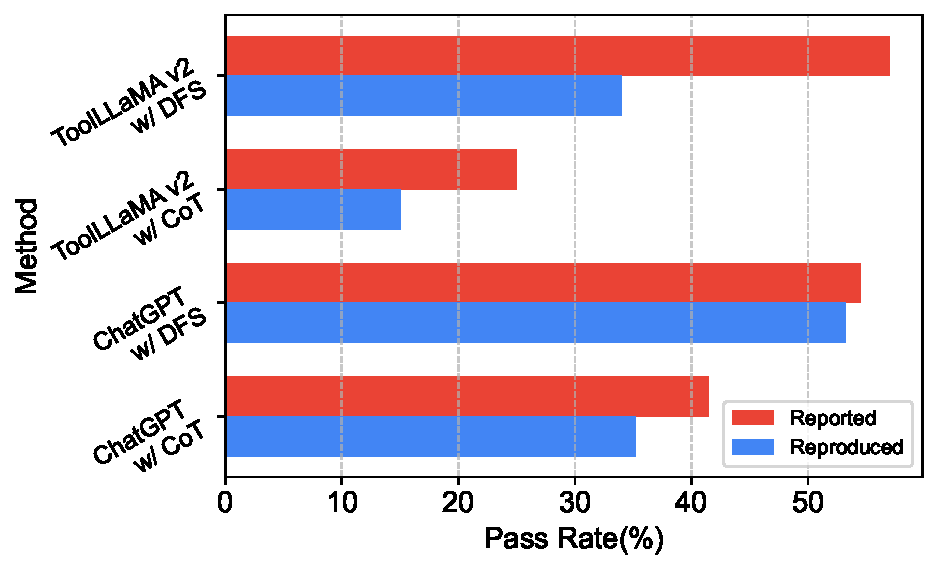
\includegraphics[width=\linewidth]{figs/real_comparison.pdf}
    \caption{Comparison of performance (Pass Rate) reported in the paper and reproduced by us on the I1-Instruction group of ToolBench.}
    \label{fig:performance_comparison_failure}
\end{figure}
The main contributions of our work are summarised as follows:
\begin{itemize}[noitemsep]
    \item A tool-learning benchmark featured a large number of cached stable simulated APIs, well-balancing stability and reality of the APIs and much more stable evaluation metrics.
    \item Extensive experiments show that our benchmark provides much more stable model performance, robust to various types of API failures.
    \item Besides enhanced stability, our virtual API system exhibits reality, diversity and reliability comparable to that of the real API system.
\end{itemize}


